%%%%%%%%%%%%%%%%%%%%%%%%%%%%%%%%%%%%%%%%%%%%%%%%%%%%%%%%%%
%%% Section 6: Experiment
%%%%%%%%%%%%%%%%%%%%%%%%%%%%%%%%%%%%%%%%%%%%%%%%%%%%%%%%%%

\section{Experimental Validation} \label{sec:c3_experiment}

\subsection{Model Validation} 

%This section compares the experimental and modelled forward progress to validate the proposed reactive ICS model. 
% As the sizing approach suggests the optimal energy storage capacitance in \SIrange{36}{46}{\micro\farad}, we select a \SI{43}{\micro\farad} capacitance in the experiment as an optimal value of the proposed sizing approach for comparison. 
% The forward progress with the optimal capacitance is compared to that with minimum and on-board ones, and an ideal case for a range of supply current. 
% Two goals:
% 1. To validate this model, to show that this model has high accuracy, so it can predict the forward progress reliably, across different energy storage capacitance and supply current. 
% 2. To show that the improvement / optimization of sizing energy storage given different current input conditions (so different energy source conditions). (Given our platform characteristics)
%\subsection{Experiment Setup}
%With the identical platform properties and workload settings in the model configuration (Section~\ref{ssubsec:loadconfig}), 
We implemented and parameterized a reactive ICS~\cite{balsamo2015hibernus} on a TI MSP430FR6989 microcontroller to validate our model. The on-board decoupling capacitance was measured as \SI{10.0}{\micro\farad}, and hence was the minimum capacitance that could be tested. Further capacitance was added to provide extra energy storage. The parameters are profiled with the MCU running a Dijkstra path finding algorithm with \SI{1696}{\byte} RAM usage at \SI{8}{\mega\hertz}. The supply voltage monitoring circuits use the MCU's internal comparator and an external \SI{3}{\mega\ohm} voltage divider. The restore and save voltage thresholds are set as $V_{r}$ = \SI{2.4}{\volt} and $V_{s}$ = \SI{2.1}{\volt} respectively. The MCU shutdown voltage $V_{off}$ is \SI{1.8}{\volt}. 


% === The following paragraph about the actually leakage is a bit weak, so removed for now. ===
% The leakage current of these capacitors was measured to be less than \SI{10}{\nano\ampere} at \SI{3}{\volt}, which is negligible compared to the \SI{}{\micro\ampere}-level current consumption of the platform; hence we omit capacitor leakage in the following experiment and model output. However, this is only applicable to the capacitors and the capacitance range in this experiment; we consider that a leakage model is still necessary for general application.
% the specific leakage current we measured does not deny that \SI{}{\micro\ampere}-level leakage may exist in most electrolytic capacitors;

% In this practical experiment, the task completion rate (i.e. tasks completed per second) is used as the metric of forward progress rather than the effective execution time ratio. To gain the task completion rate from the model, we multiply the normalized forward progress (execution time ratio) generated from our model by the completion rate when the system executes constantly, since the task completion rate is linear to the effective execution time. 

%\subsection{Validation Results}
\begin{figure}
	\centering
	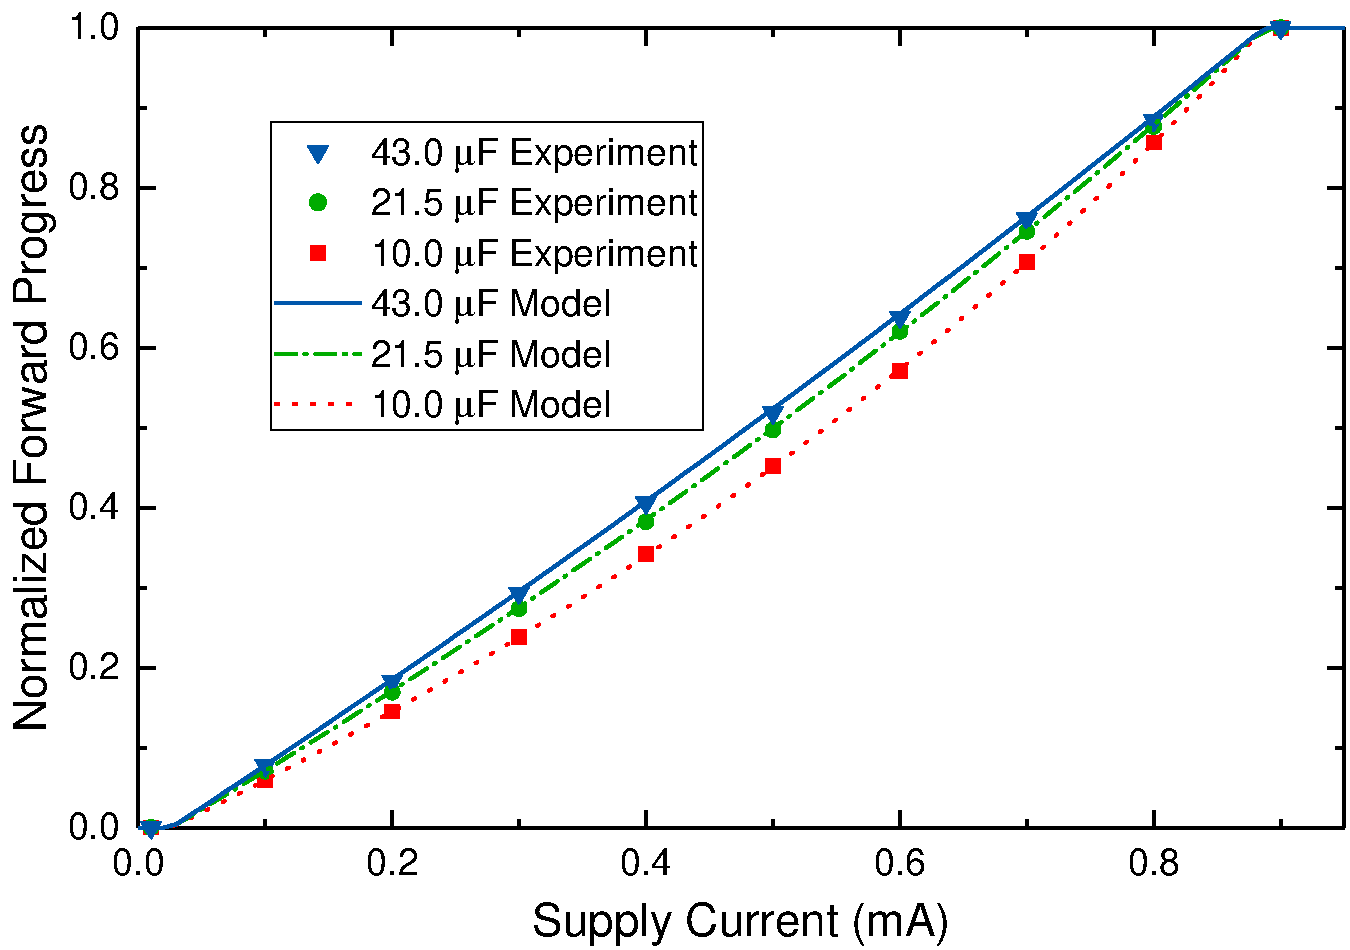
\includegraphics[width=0.8\columnwidth]{ch3_sizingeffect/figures/ModelValidFig} % was 3.0in
	\caption{Model validation with experimental and modelled forward progress. }
	\label{fig:modelvalid}
\end{figure}

% Validate the formulation and test the error/accuracy of the model. 
To validate the accuracy of our model, we powered the device with a range of supply currents ([0.1, 0.2, ..., 0.8]\SI{}{\milli\ampere}) to operate the device in \textit{Intermittent} mode, and repeated the tests with three energy storage capacities: a) \SI{10.0}{\micro\farad} decoupling capacitance; b) \SI{21.5}{\micro\farad} (\SI{11.5}{\micro\farad} added); c) \SI{43.0}{\micro\farad} (\SI{33.0}{\micro\farad} added). We compared the actual forward progress against predictions generated from our model. As shown in \figurename{~\ref{fig:modelvalid}}, the model-generated output matches closely with the experimental results with only 0.5\% mean absolute percentage error. 
% Hence, the model is able to accurately estimate forward progress for design exploration. 

% I think I need a bit more reasonable discussion here to argue. 

% Properly sizing energy storage benefits forward progress. 
% We compared the tested completion speed among the minimum capacitance (\SI{6.2}{\micro\farad}, model generated), the on-board \SI{10}{\micro\farad} case, the efficient \SI{43}{\micro\farad} case, and an ideal case. 

% Using a larger capacitor improves forward progress.
% Reduction of state saving and restoring overheads and forward progress improvement. 

% \begin{figure}[!t]
%     \centering
%     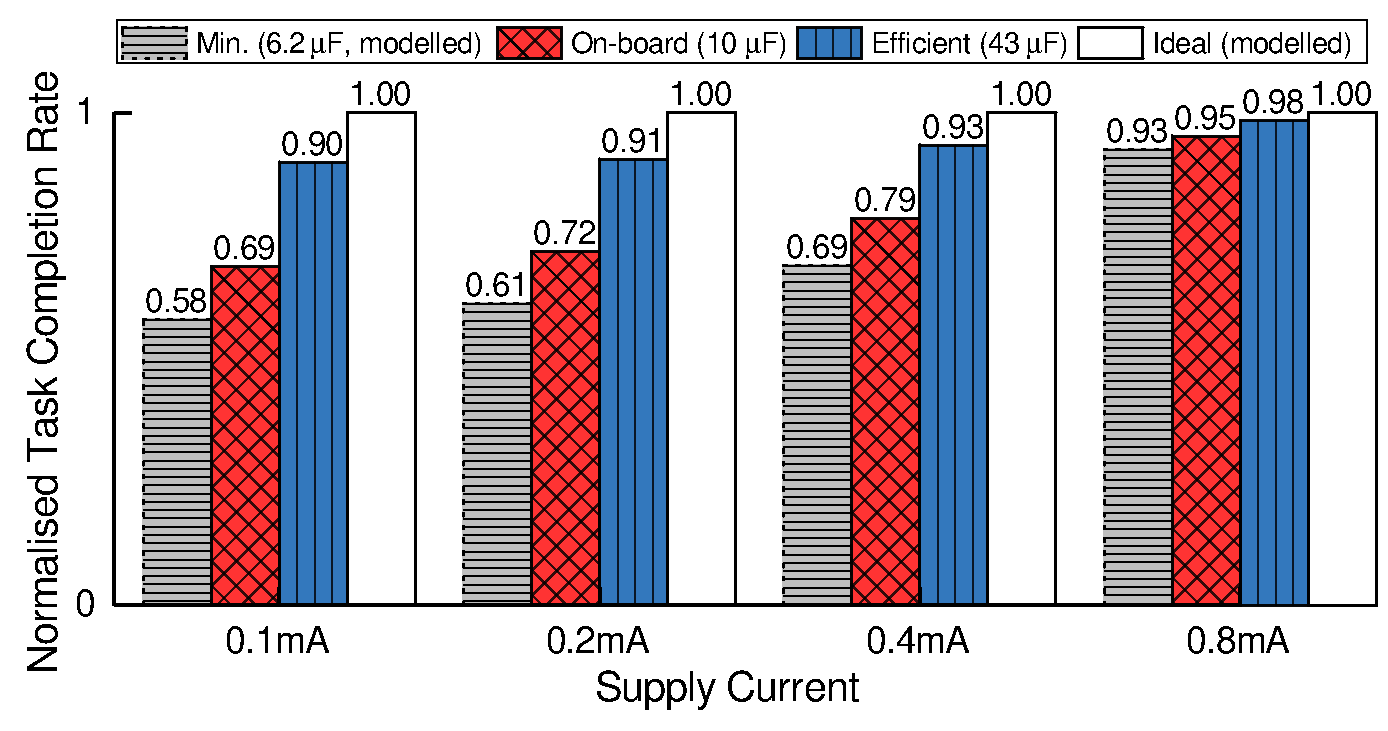
\includegraphics[width=3.33in]{ImprValidFigColor}
%     \caption{Experimental comparison of task completion rates (forward progress) given different energy storage capacities. }
%     \label{fig:imprvalid}
% \end{figure}

\subsection{Validation of Sizing Effects}

We show with modelled and experimental results that (\fref{fig:imprvalid1}) using efficiently-sized energy storage capacitance (\SI{43}{\micro\farad}) achieves up to a 55\% improvement in forward progress compared against using the theoretical minimum amount of capacitance (\SI{6.2}{\micro\farad}). 
This improvement is more significant with a weaker supply. 

\begin{figure}
    \centering
    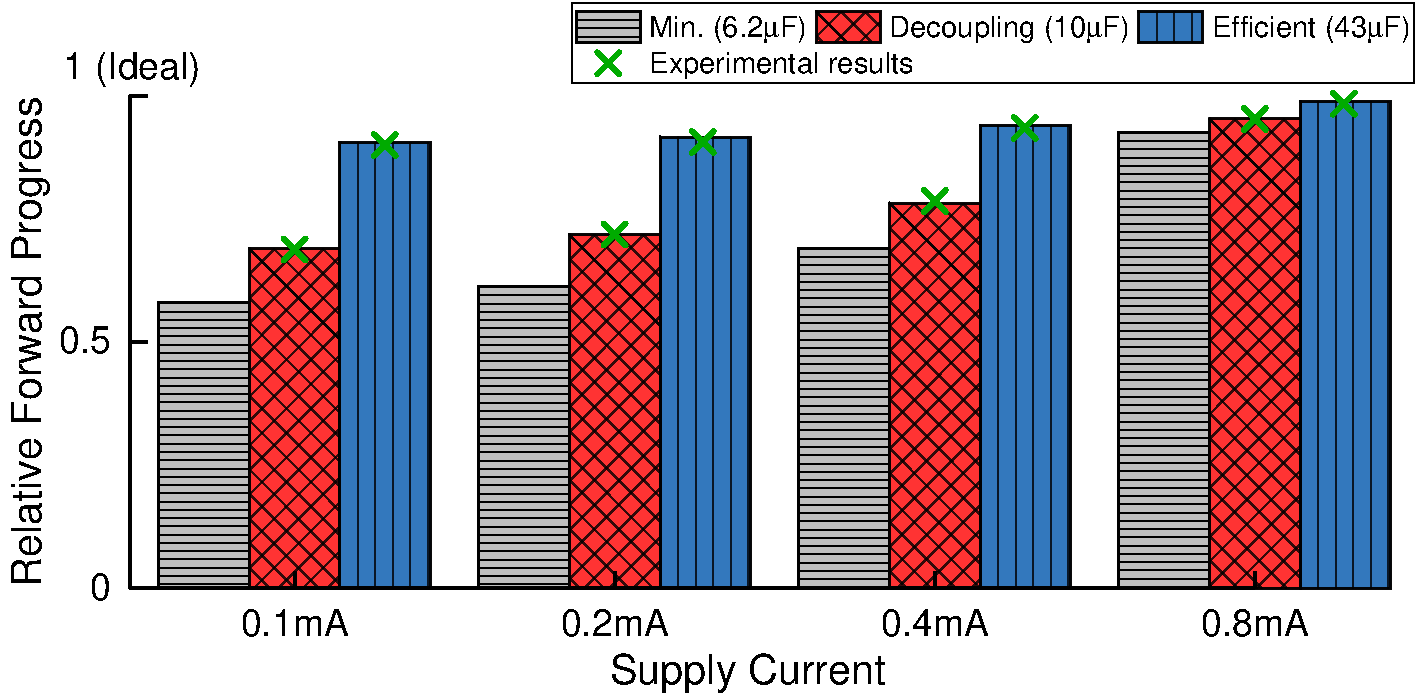
\includegraphics[width=\columnwidth]{ch3_sizingeffect/figures/ImprValidColorFig1}
    \caption{The relationship between energy storage capacitance and IPS forward progress, for various supply currents. }
    \label{fig:imprvalid1}
\end{figure}

As previously shown in Fig.\ref{fig:imprvalid1}, the efficiently-sized energy storage capacitance (\SI{43}{\micro\farad}) improves forward progress by up to 55\% and 30\% compared to the minimum and decoupling capacitance respectively. We notice that this improvement becomes significant when the supply current attenuates because the save and restore overheads consume a larger proportion of the available energy. Also, this achieves at least 90\% of the ideal forward progress mentioned in Section~\ref{subsec:formulation}. 
% The ideal case switches between LPM and execution without restoring and saving overheads (mentioned in Section~\ref{subsec:formulation}). 
These results illustrate the importance of this technique, in particular for conditions where the supply current is low.